\documentclass[11pt]{beamer}
\usetheme{metropolis}

\usepackage[utf8]{inputenc}
\usepackage[spanish]{babel}
\usepackage[T1]{fontenc}

\usepackage{amsmath}
\usepackage{amsfonts}
\usepackage{amssymb}
\usepackage{graphicx}
\usepackage{url}
\usepackage{booktabs}
\usepackage{graphicx}
\usepackage[table]{xcolor}
\usepackage{comment}
\usepackage{multimedia}
\usepackage{fontawesome5}


\DeclareMathOperator{\sen}{sen}
\DeclareMathOperator{\tg}{tg}

\setbeamertemplate{caption}[numbered]


\title[ST: Mapudungún]{Low resource speech translation}
\subtitle{Una arquitectura de \textit{fine-tuning} eficiente para el Mapudungún}
\author[Barriga]{
    Diego Barriga, Edgar Gazque \\
    \texttt{dbarriga@ciencias.unam.mx}, \texttt{amilkar@ciencias.unam.mx} \\
}
\institute[UNAM]{
    Procesamiento del Lenguaje Natural \\
    Programa de Posgrado en Ciencia e Ingeniería de la Computación (PCIC)\\
    Universidad Nacional Autónoma de México
}
\date{25 de Mayo 2026}

\titlegraphic{
    \begin{minipage}{\textwidth}
        %\raggedright
        %
\includegraphics[width=0.5cm]{img/unam.png}
        %\hfill
        
\includegraphics[width=1.5cm]{img/unam.png}
        \raggedleft
    \end{minipage}
}

\setbeamertemplate{navigation symbols}{}


\newcommand{\email}{email}

% La agenda se mostrará al inicio de cada sección
\AtBeginSection[]
{
  \begin{frame}
    \frametitle{Table of Contents}
    \tableofcontents[currentsection]
  \end{frame}
}

\begin{document}

\begin{frame}
\titlepage
\end{frame}

\begin{frame}{Contenido}
\tableofcontents
\end{frame}

\section{Traducción automática}

\begin{frame}{Antecedentes}

    \begin{itemize}
        \item <1-> La traducción automática (\textit{Machine Translation, MT}) es una tarea del Lingüística Computacional icónica.
        \item <2-> La primera demostración pública de un sistema de traducción automática data de 1954\footnote{\url{https://www.nytimes.com/1954/01/08/archives/russian-is-turned-into-english-by-a-fast-electronic-translator.html}}
        \item <3-> El reporte \textit{ALPAC, Automatic Language Processing Advisory Committee} de 1966 concluyó que la traducción automática no era viable.
    \end{itemize}
\end{frame}

\begin{frame}
    \begin{figure}
        \centering
        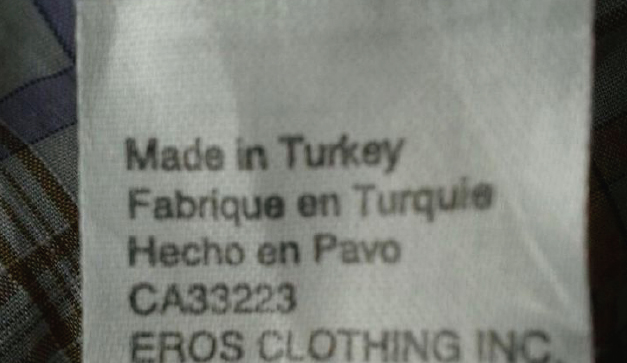
\includegraphics[width=\textwidth]{img/translation_2.jpg}
    \end{figure}
\end{frame}

\begin{frame}{Adopción de la tecnología}
    \begin{figure}
        \centering
        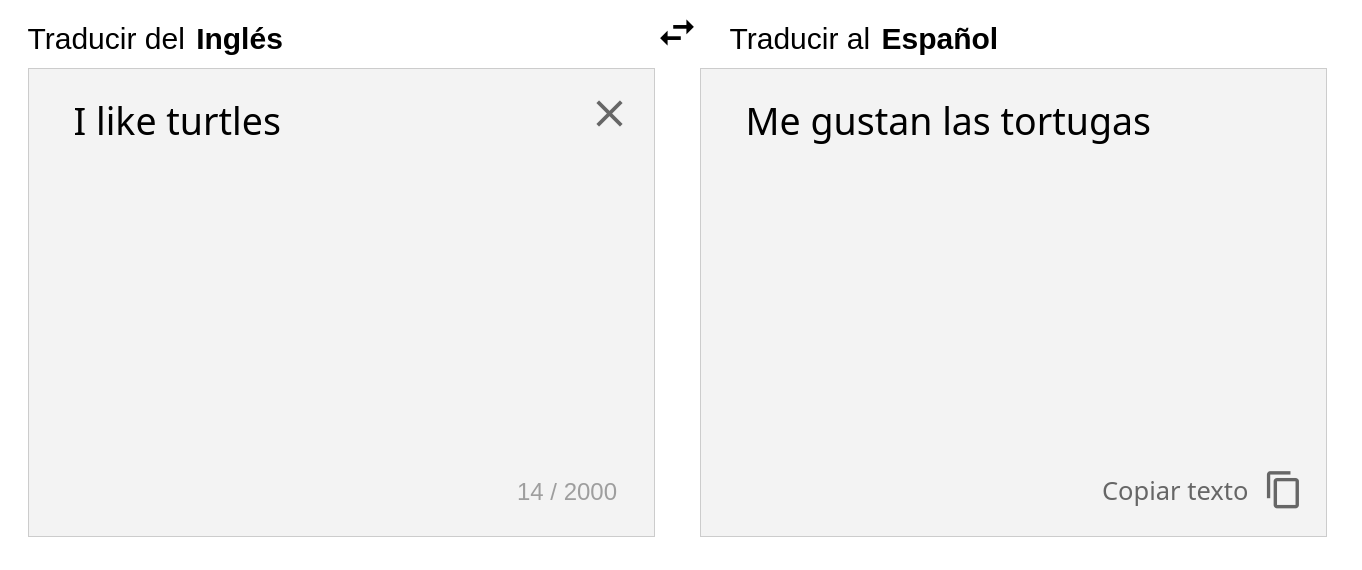
\includegraphics[width=\textwidth]{img/translate.png}
        \caption{Traducción automática en un servicio en línea \url{https://libretranslate.com/}.}
    \end{figure}
\end{frame}

\begin{frame}{Reconocimiento automático del habla}
    \begin{itemize}
        \item El reconocimiento automático del habla (\textit{Automatic Speech Recognition, ASR}) es una tarea que busca convertir audio en texto.
        \item Se utiliza en aplicaciones como asistentes de voz, transcripción de reuniones, y sistemas de dictado.
    \end{itemize}
\end{frame}

\begin{frame}
    \begin{figure}
        \centering
        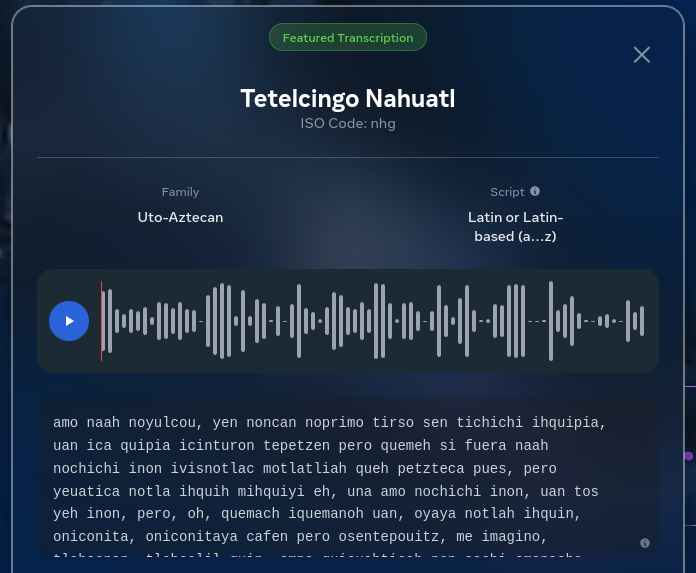
\includegraphics[width=0.8\textwidth]{img/asr.png}
        \caption{Ejemplo de sistema de reconocimiento automático del habla. Tomada de \url{https://aidemos.atmeta.com/omnilingualasr/language-globe}}
    \end{figure}
\end{frame}

\begin{frame}{Traducción automática del habla}
    \begin{itemize}
        \item La traducción automática del habla (\textit{Speech Translation, ST}) es una tarea que combina el reconocimiento automático del habla (\textit{Automatic Speech Recognition, ASR}) con la traducción automática (\textit{MT}).
        \item El objetivo es traducir el \textbf{audio de una lengua a texto en otra lengua}.
    \end{itemize}
\end{frame}

\begin{frame}
    \begin{figure}
        \centering
        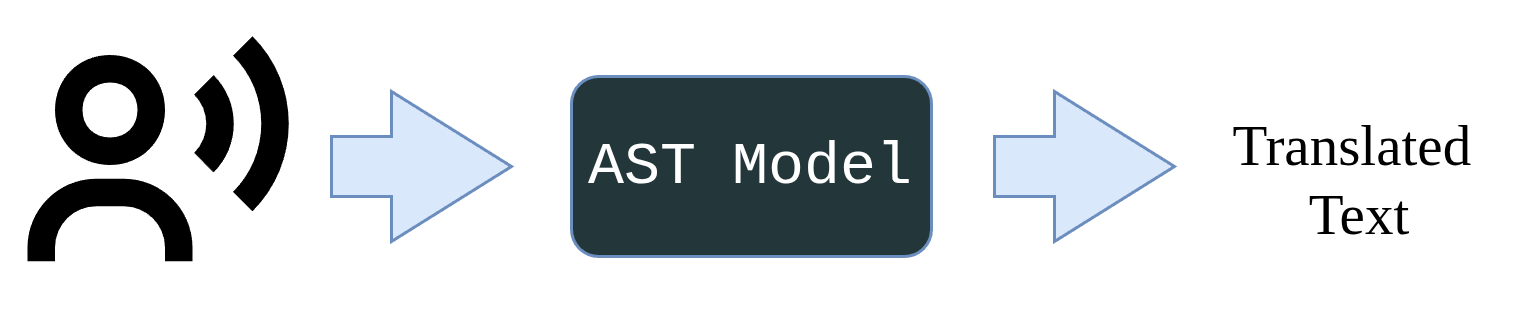
\includegraphics[width=\textwidth]{img/ast_diagram.png}
        \caption{Ejemplo de sistema de traducción automática del habla. Ingresa audio en una lengua y sale texto en otra lengua.}
    \end{figure}
\end{frame}

\begin{frame}{Modelos Masivos}
    \begin{itemize}
        \item <1-> En los últimos años, se ha optado por utiliza un enfoque \textit{encoder-decoder} basado en redes neuronales profundas, con modelos como Transformers \cite{vaswani2017attention}.
        \item <2-> En particular, se aprovechan modelos masivos pre-entrenados de forma \textit{\textbf{end-to-end}} para tareas de traducción automática y reconocimiento del habla.
        \item <3-> Estos modelos aprenden a mapear de un audio a su representación textual.
        \item <4-> Para adaptar estos modelos a tareas específicas, se utiliza el \textbf{ajuste fino} (\textit{fine-tuning}), donde se entrena el modelo con un conjunto de datos específico para la tarea.
    \end{itemize}
\end{frame}

\begin{frame}
    \begin{figure}
        \centering
        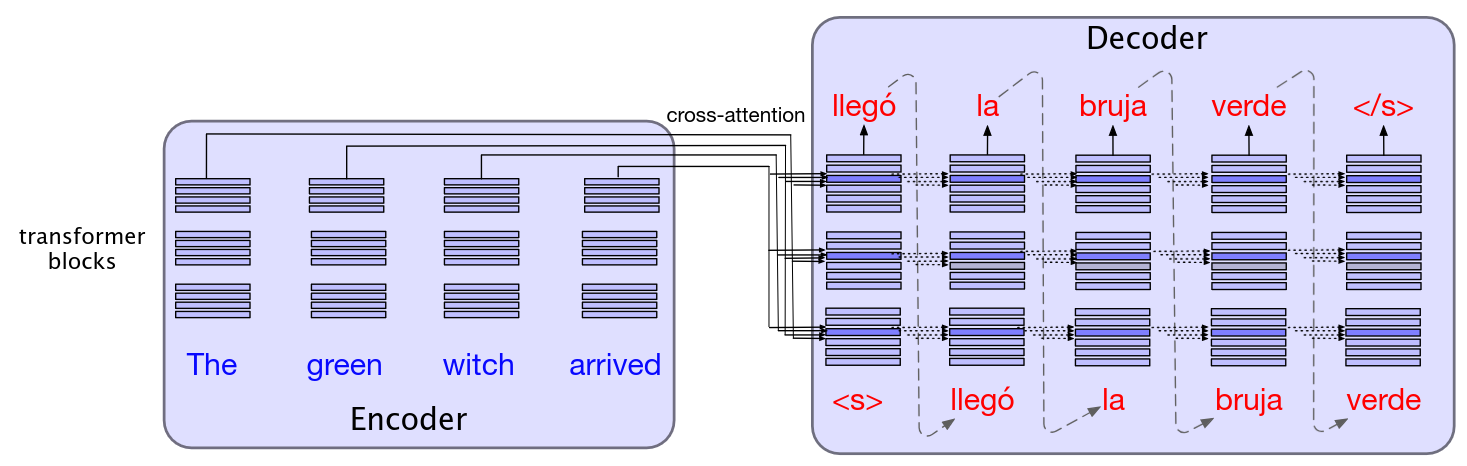
\includegraphics[width=\textwidth]{img/seq2seq.png}
        \caption{Arquitectura \textit{encoder-decoder} para traducción automática. Tomada de \cite{jm3}}
    \end{figure}
\end{frame}

\begin{frame}{¿Qué es End-to-End Speech Translation?}

    \begin{block}{Enfoque clásico}
        \begin{center}
            Audio $\rightarrow$ \fbox{ASR} $\rightarrow$ Texto Transcrito $\rightarrow$ \fbox{MT} $\rightarrow$ Texto Traducido
        \end{center}
        \small
        \textit{Problema: Propagación de errores.}
    \end{block}
    
    \begin{block}{Enfoque directo (\textit{end-to-end})}
        \begin{center}
            Audio $\rightarrow$ \fbox{\textbf{Modelo Único}} $\rightarrow$ Texto Traducido
        \end{center}
        \small
        \textit{Ventaja: Menor latencia, no requiere transcripciones intermedias en entrenamiento.}    
    \end{block}
    
    
\end{frame}

\section{Problemática}

\begin{frame}{Diversidad lingüística en América Latina}

    \begin{itemize}
        \item <1-> América Latina es una región con una gran diversidad lingüística, albergando cientos de lenguas originarias.
        \item <2-> Limitandonos a México, existen 68 lenguas originarias reconocidas oficialmente, con más de 360 variantes dialectales.
        \item <3-> Todas las lenguas originarias de México son de \alert{bajos recursos digitales}. Una realidad para muchas lenguas originarias en América Latina.
        \item <4-> Hay muy poca tecnología del lenguaje desarrollada para estas lenguas.
        \item <5-> La mayoría de las lenguas originarias no tienen sistema de escritura estandarizado. Son \alert{lenguas principalmente orales}.
    \end{itemize}

\end{frame}

\begin{frame}

    \begin{figure}
        \centering
        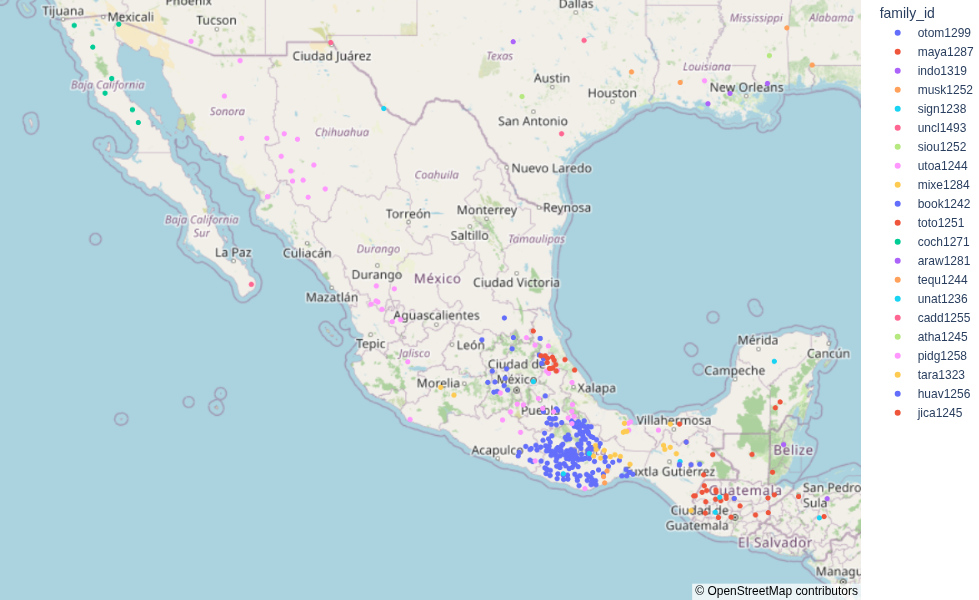
\includegraphics[width=\textwidth]{img/mex_map.png}
        \caption{Lenguas originarias de México. Tomada de la \href{https://github.com/umoqnier/cl-2026-2-lab/blob/main/practicas/romanbott/P2/Practica2.ipynb}{práctica 2} del Lingüística Computacional del alumno \texttt{@romanbott}}
    \end{figure}
    
\end{frame}


\begin{frame}{Reto principal}

 \Large Los modelos estándar de \textit{encoder-decoder} usando \textit{transformers} requieren miles de horas de audio alineado. Las lenguas originarias \textbf{carecen de estos recursos}.

\end{frame}

\begin{frame}{Preguntas de Investigación:}

\begin{enumerate}
    \item <1-> ¿Es posible \textbf{transferir conocimiento} de modelos masivos pre-entrenados en lenguas mayoritarias hacia lenguas con tipologías drásticamente distintas como las lenguas originarias?
    \item <2-> ¿Un entrenamiento \textit{end-to-end} tendrá un \textbf{mejor desempeño que un sistema de cascada} (ASR + MT) en este entorno de bajos recursos?
    \item <3-> ¿Qué técnicas de ajuste eficiente de parámetros son efectivas en este entorno?
    \item <4-> ¿Un enfoque de entrenamiento multilingüe mejora el rendimiento individual al \textbf{compartir características} acústicas/semánticas?
\end{enumerate}

\end{frame}

\section{Especificaciones del reto}

\begin{frame}{Contexto: IWSLT 2026}
\begin{columns}
    \begin{column}{0.6\textwidth}
        \textbf{International Conference on Spoken Language Translation}\footnote{\url{https://iwslt.org/2026/low-resource}}
        \begin{itemize}
            \item Conferencia anual líder en evaluación de sistemas de traducción de habla.
            \item Organiza \textit{Shared Tasks} (tareas compartidas) para benchmark global.
            \item Fomenta la publicación de descripciones de sistemas y hallazgos científicos.
        \end{itemize}
    \end{column}
    \begin{column}{0.4\textwidth}
        \centering
        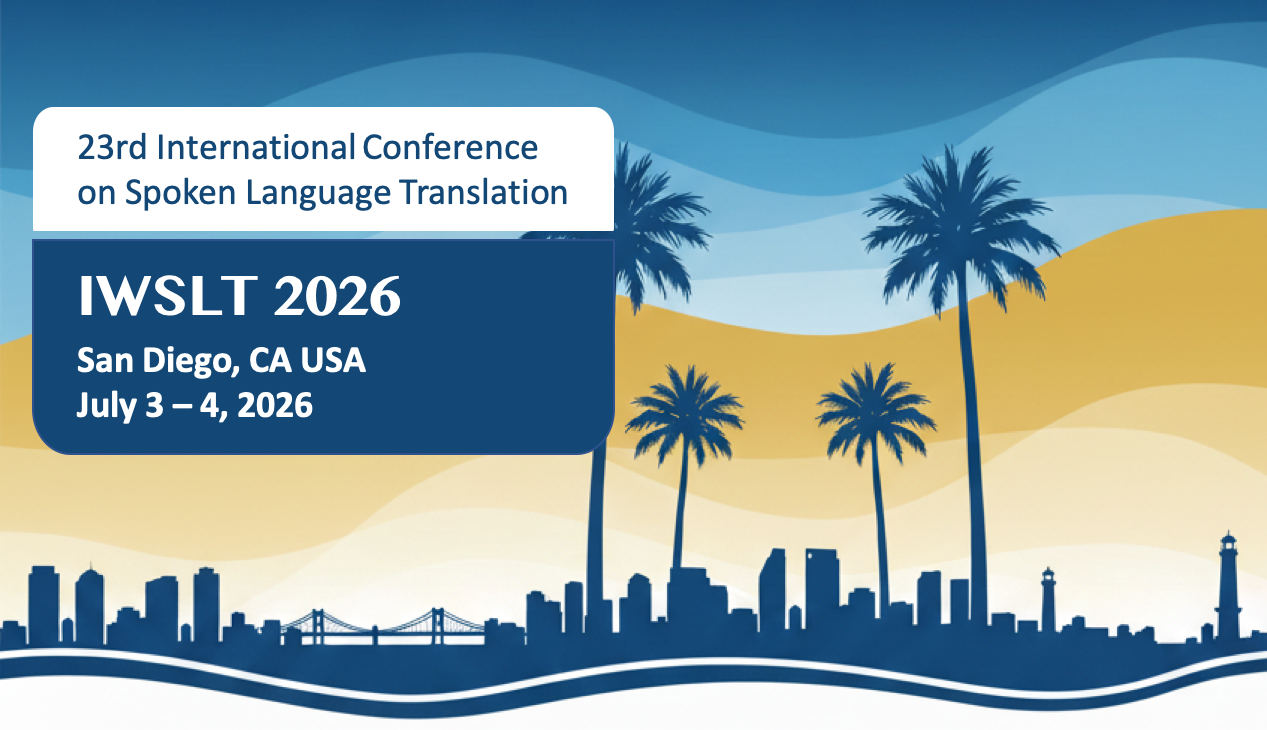
\includegraphics[width=1.0\linewidth]{img/iwslt2026_logo.png}
    \end{column}
\end{columns}
\end{frame}

\begin{frame}{Nuestra Participación: \textit{Low-Resource} Track}

    \begin{itemize}
        \item <1-> \textbf{Objetivo General:} El objetivo es evaluar y promover tecnologías de la traducción del habla (\textit{speech translation, ST}) donde los datos son escasos.
        \item <2-> Participamos en el \textit{shared task} enfocado en lenguas de \textbf{bajos recursos digitales} (\textit{low-resource languages}).
    \end{itemize}

\end{frame}

\begin{frame}{Track 1: Speech to text translation}

\begin{itemize}
    \item <1-> Realizamos un sistema de \textit{speech translation} para el track 1 el cual contempla 10 lenguas topológicamente diversas.
    \item <2-> Nos enfocamos en lenguas habladas en América Latina, en partícula, \textbf{realizamos un sistema monolingüe} Mapuche $\rightarrow$ Español.
\end{itemize}

\end{frame}


\section{Propuesta}

\begin{frame}{Ajuste fino (\textit{Fine-Tuning})}

    \begin{itemize}
        \item <1-> El ajuste fino es una técnica de transferencia de aprendizaje donde un modelo pre-entrenado se adapta a una tarea específica con un conjunto de datos más pequeño.
        \item <2-> Los modelos masivos pre-entrenados ya han aprendido representaciones lingüísticas generales, el ajuste fino es una estrategia para adaptar estos modelos a tareas específicas con pocos datos.
    \end{itemize}
\end{frame}

\begin{frame}

    \begin{figure}
        \centering
        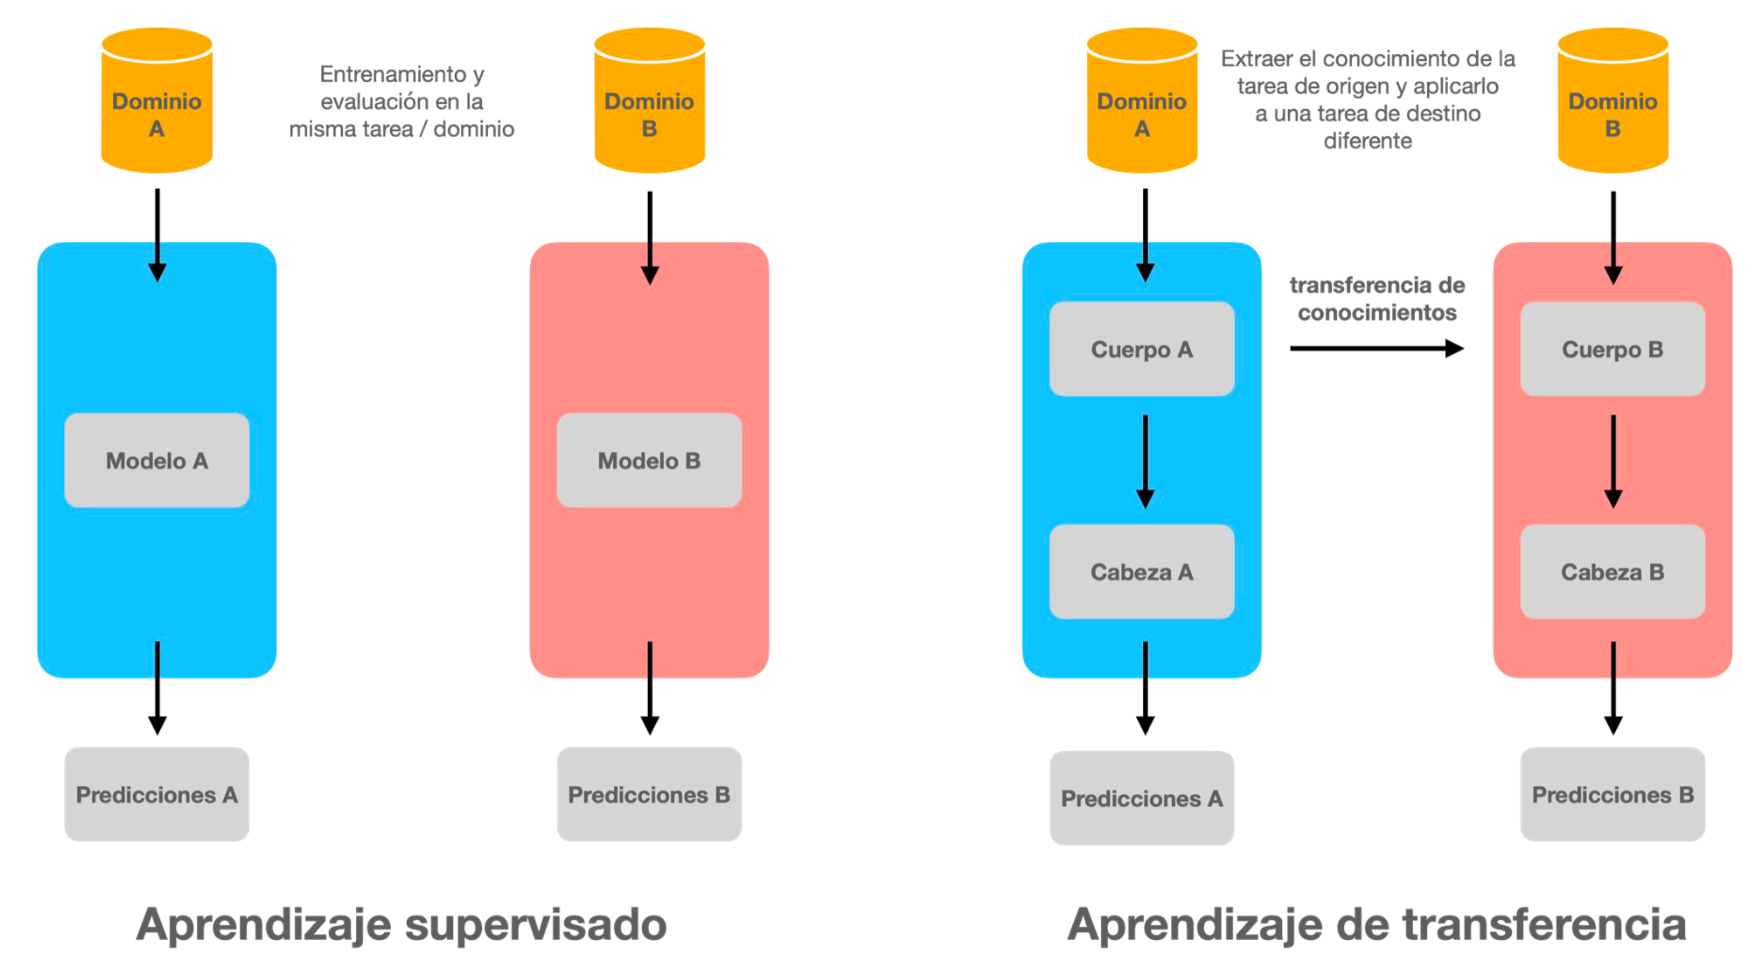
\includegraphics[width=\linewidth]{img/fine_tuning.png}
        \caption{Transferencia de conocimiento de un modelo pre-entrenado a otra tarea. Tomada de clase 7 del curso Analítica de Textos y Modelos de Lenguaje derivada de \url{https://somosnlp.org/nlp-de-cero-a-cien/sesion-04}.}
    \end{figure}

\end{frame}

\begin{frame}{Fine-tuning Eficiente (PEFT)}
   En el contexto de los bajos recursos, un \textit{Full Fine\-Tuning} causaría \textbf{overfitting} y es computacionalmente costoso.

    \begin{figure}
        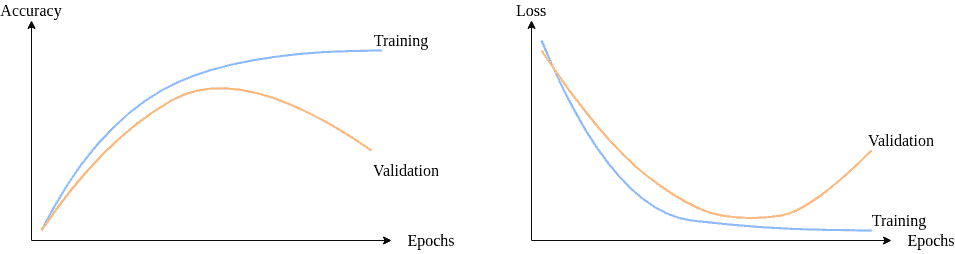
\includegraphics[width=\linewidth]{img/overfitting.png}
    \end{figure}

    Nuestra propuesta: \pause \textbf{Parameter-Efficient Fine-Tuning (PEFT) \cite{xu2023parameterefficientfinetuningmethodspretrained}}
\end{frame}

\begin{frame}{Houlsby Adapter \cite{DBLP:journals/corr/abs-1902-00751}}
    En la implementacion llamado \textit{Linear adapter} 
    \begin{figure}
        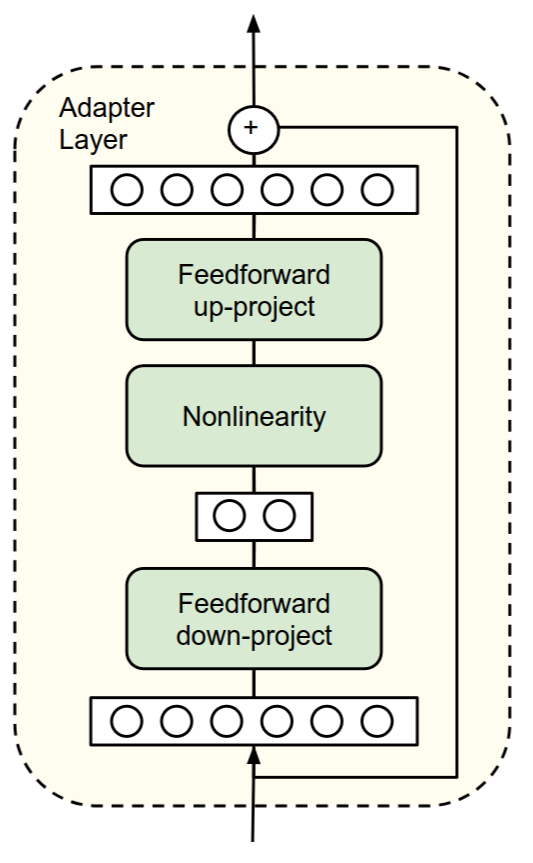
\includegraphics[width=0.3\linewidth]{img/Adapter.png}
    \end{figure}
    Caracteristicas: Modulo Linear Feedforward, LayerNorm, Una sola capa oculta con funcion de activacion.
\end{frame}

\begin{frame}{Caracteristicas del adapter \cite{DBLP:journals/corr/abs-2110-04366}}
    \begin{itemize}
        \item \textbf{Funcional:} Los parametros entrenables que modificaran el \textit{input}
        \item \textbf{Inserción:} Las salidas del adaptador se integran con la entrada original.
        \item \textbf{Composición:} Cómo se integran las salidas de los adaptadores con las entradas. Ejemplo  una conexión de suma residual o multiplicacion elemento a elemento.
    \end{itemize}   
\end{frame}

\begin{frame}{Adapters para ST de lenguas originarias}

    \begin{itemize}
        \item <1-> Se congelan la mayoría de los pesos de un modelo preentrenado (ej. \texttt{canary-1b-v2}).
        \item <2-> Se habilitan pequeñas capas entrenables.
        \item <3-> \textbf{Estrategia específica:} Entrenaremos adapters en el \textit{Encoder} para capturar la acústica de las nuevas lenguas.
        \item <4-> Con esta configuracion entrenamos \texttt{589,824} parametros de un total de \texttt{962,745,344}, es decir menor al 0.1 \% 
    \end{itemize}

\end{frame}

\begin{frame}{Modelos pre-entrenados: Canary}

    Canary 1B v2 \cite{koluguri2025granaryspeechrecognitiontranslation}. Un modelo de \textit{1 Billon} de parámetros entrenado con al rededor de 1.7 millones de horas de 25 idiomas. En este trabajo también se entreno con lenguas de bajos recursos como Lituano.

    \begin{figure}
    
\includegraphics[width=0.5\linewidth]{img/nvidia-logo-horz.png}
    \end{figure}
\end{frame}

\begin{frame}{Canary como modelo base}

    \begin{itemize}
        \item <1-> Canary es un modelo de tipo \textit{encoder-decoder} basado en la arquitectura Conformer \cite{gulati2020conformerconvolutionaugmentedtransformerspeech} y en particular en la variante Fast Conformer \cite{rekesh2023fastconformerlinearlyscalable}.
        \item <2-> Fue entrenado de forma multilingüe y multitarea (\textit{ASR} y \textit{ST})
        \item <3-> El modelo original fue entrenado con 1.7 millones de horas de audio en 22 idiomas de grandes recursos y 3 idiomas de bajos recursos.
        \item <4-> Utilizamos este modelo para realizar una \alert{corrida experimental inicial}.
    \end{itemize}
\end{frame}

\begin{frame}{Arquitectura}
    \begin{figure}
        \centering
        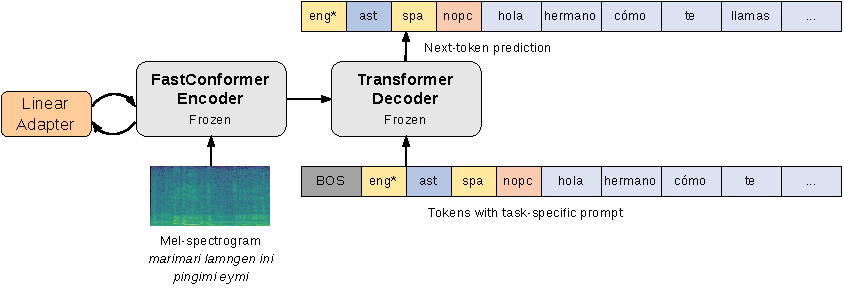
\includegraphics[width=\linewidth]{img/canary_and_linear_adapter.pdf}
        \caption{Arquitectura de Canary con Adapters lineales. Código en \url{https://github.com/umoqnier/iwstl-low-resource-experiments/}}
    \end{figure}
\end{frame}

\section{Corpus}

\begin{frame}{Mapuche (Mapudungún)}
\begin{itemize}
    \item \textbf{Familia:} Araucana.
    \item \textbf{Hablantes:} 100K - 260K \cite{zuniga2006mapudungun}.
    \item \textbf{Países:} Chile, Argentina.
    \item  \textbf{Características:} Lengua no clasificada \cite{zuniga2006mapudungun}.
\end{itemize}
\end{frame}

\begin{frame}{Estadísticas del Dataset (IWSLT proporcionado)}
    
    \begin{center}
    \begin{tabular}{lrr}
        \toprule
        \textbf{Métrica} & \textbf{Mapuche} \\
        \midrule
        Horas de Audio & \textbf{90} \\
        Frases Alineadas & 42,000 \\
        Dominio & Narraciones, histórico \\
        \bottomrule
    \end{tabular}    
    \end{center}
\end{frame}

\begin{frame}{Características del Texto (Mapudungun)}
    \setbeamerfont{caption}{size=\tiny} 

    \begin{columns}[t]
        \begin{column}{0.32\textwidth}
            \centering
            \begin{figure}
                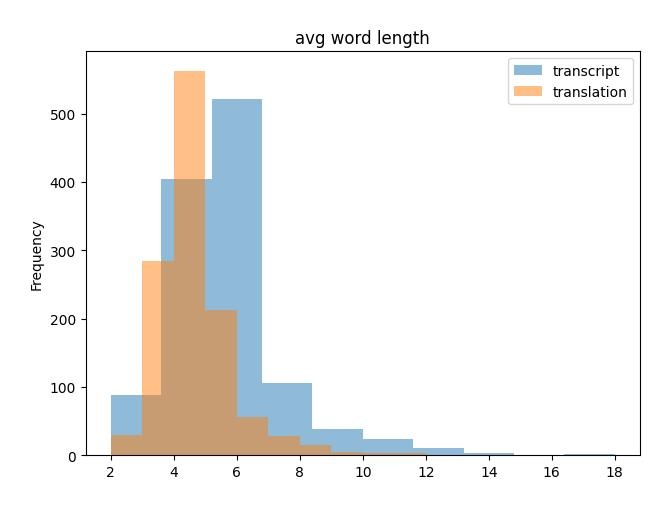
\includegraphics[width=\textwidth]{img/Graficas/mapuche/avg_word_length.jpg}
                \caption{Longitud de palabra}
            \end{figure}
        \end{column}

        \begin{column}{0.32\textwidth}
            \centering
            \begin{figure}
                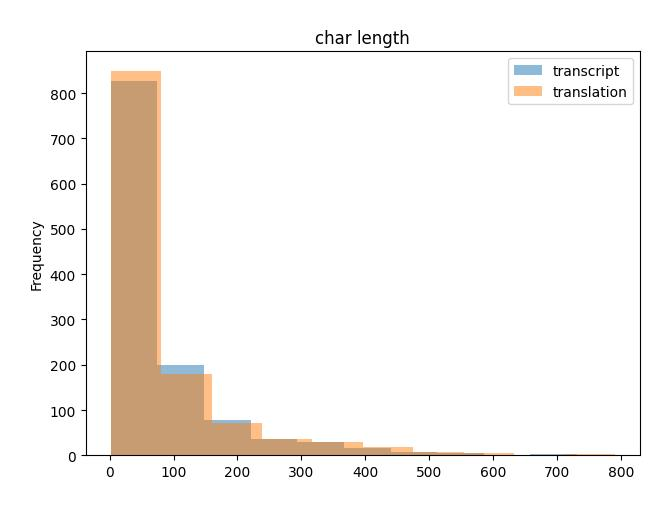
\includegraphics[width=\textwidth]{img/Graficas/mapuche/char_length.jpg}
                \caption{Longitud de caracteres}
            \end{figure}
        \end{column}

        \begin{column}{0.32\textwidth}
            \centering
            \begin{figure}
                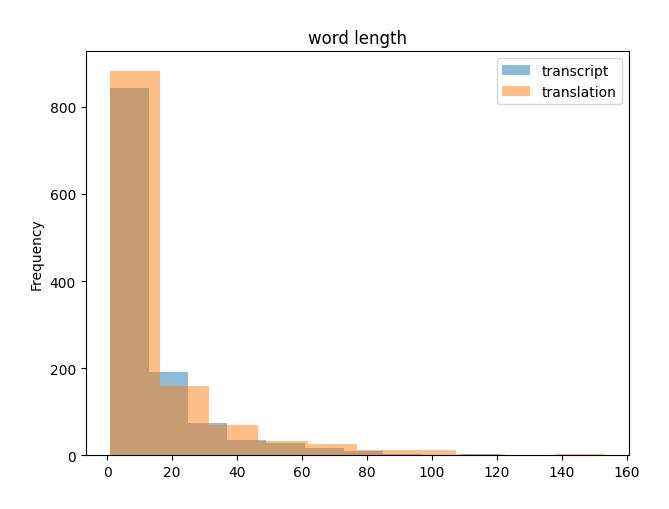
\includegraphics[width=\textwidth]{img/Graficas/mapuche/word_length.jpg}
                \caption{Longitud de oración}
            \end{figure}
        \end{column}
    \end{columns}
\end{frame}

\begin{frame}{Aumentación de datos}

    \begin{block}{Pipeline dinámico}
        \begin{itemize}
            \item Implementación de un flujo de aumentación de datos de forma \textit{on-the-fly} basado en \cite{audiomentations}.
            \item Aplicado directamente durante el entrenamiento.
            \item Eliminamos la necesidad de almacenar datos pre-procesados adicionales.
        \end{itemize}
    \end{block}
    
    \begin{block}{Tecnicas estocásticas}
        \begin{itemize}
            \item Inyección de ruido de fondo y ruido gaussiano.
            \item Aplicación de \textit{aliasing} y respuestas al impulso de sala (\textit{room impulse responses}).
            \item Filtrado de paso banda (\textit{band-pass filtering}).
            \item Desplazamiento de tono (\textit{pitch shifting}).
        \end{itemize}
    \end{block}
\end{frame}

\begin{frame}
    \begin{exampleblock}{Ejemplo}
        \begin{itemize}
            \item \movie[externalviewer]{\textcolor{blue}{$\blacktriangleright$ \ Audio}}{audio/sample.wav} $\rightarrow$ coñoepan soy yo aquí en esta tierra nací tierra de cahuemu isla huapi se llama
        \end{itemize}
        
    \end{exampleblock}
     
\end{frame}

\section{Resultados}

\begin{frame}{Resultados}
    \begin{itemize}
        \item <1-> El \textit{Word Error Rate, WER} y el \textit{BLEU} de entrenamiento decreció como se esperaba.
        \item <2-> Agregamos un modulo de aumentación de datos que \alert{no ayudó} a mejorar el desempeño.
        \item <3-> Un análisis cualitativo muestra que el modelo si alcanza a capturar fenomenos del habla del Mapudungún. Ver ejemplo \ref{example:good}.
        \item <4-> Sin embargo, el modelo tiende a caer en la repetición de estructuras básicas del español. Ver ejemplo \ref{example:bad}.
    \end{itemize}
\end{frame}

\begin{frame}{Métricas}
    \begin{table}
        \begin{center}
            \begin{tabular}{|l|c|c|}\hline
            Run & WER on dev & BLUE on dev\\\hline
            Main &  $2.5$       & $1.015$ \\
            Vanilla & $2.3$     & $1.05$  \\
            Filtered & \textbf{$1.56$}  & \textbf{$3.7$}\\\hline
            \end{tabular}
            \caption{\textbf{Main:} Corrita principal, incluye el modulo de aumentación de datos. \textbf{Vanilla:} No incluye aumentación de datos. \textbf{Filtered:} Corrita sin el modulo de aumentación de datos y con los audios de menos de 15 segundos. El resto de audios fue usado para pruebas.}
            \label{tbl:results}
        \end{center}
    \end{table}
\end{frame}

\begin{frame}{Main}
    \begin{figure}
        \centering
        
\includegraphics[width=0.9\linewidth]{img/Resultados/3/training_batch_wer_vs_val_wer.png}
        \caption{Corrida experimental principal. Incluye el modulo de aumentación de datos.}
    \end{figure}
\end{frame}

\begin{frame}{Filtrado I}
    \begin{figure}
        \centering
        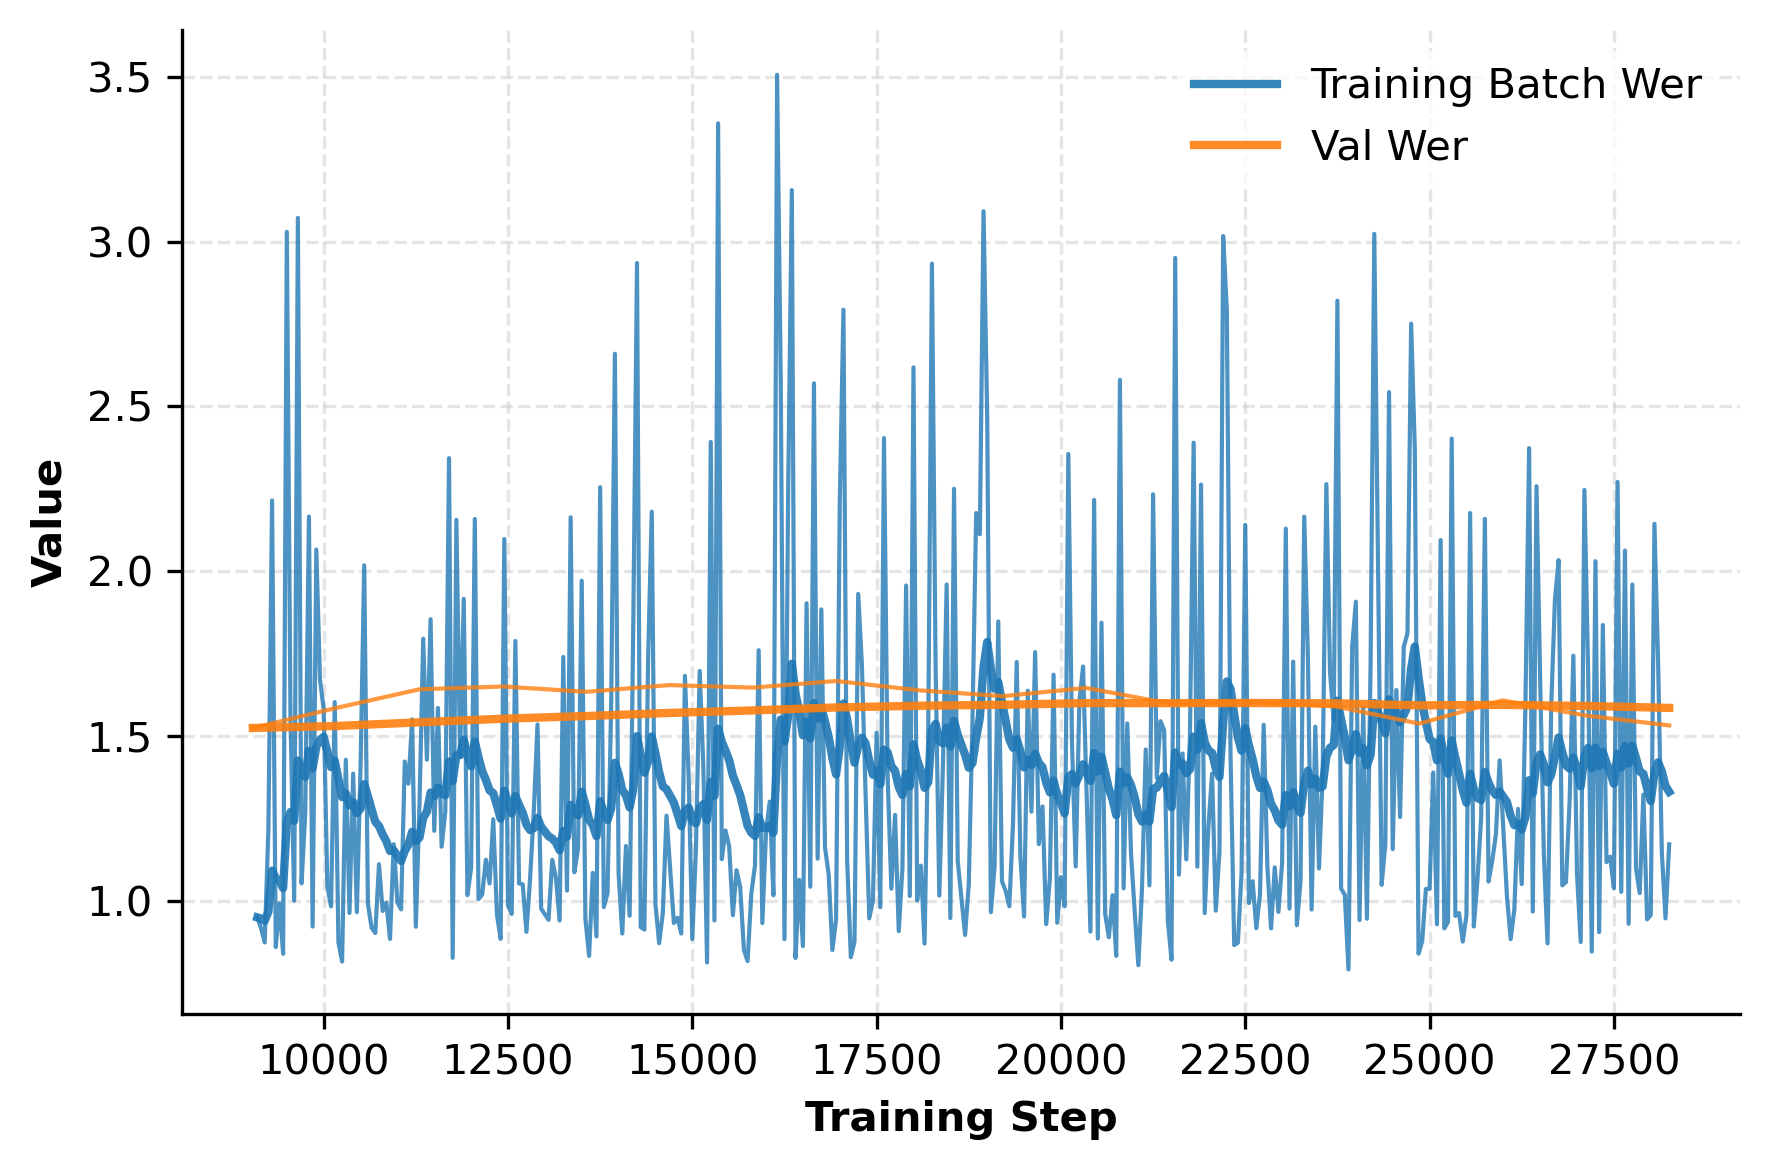
\includegraphics[width=0.9\linewidth]{img/Resultados/100/training_batch_wer_vs_val_wer.png}
        \caption{Corrida experimental con audios filtrados.}   
    \end{figure}
\end{frame}

\begin{frame}{Filtrado II}
    \begin{figure}
        \centering
        
\includegraphics[width=0.9\linewidth]{img/Resultados/12/training_batch_wer_vs_val_wer.png}
        \caption{Corrida experimental con audios filtrados y con el modulo de aumentación de datos.}
    \end{figure}
\end{frame}



\begin{frame}{Ejemplos}
    \begin{enumerate}
        \item \textbf{Transcripción adecuada de palabras raras} \label{example:good}
        \begin{quote}
            \textit{Referencia:} sí pero yo creo que hay eso sí que no sé pero en las cosas del huinca parece que hay una tableta \\
            \textit{Predicción:} sí pero yo creo que hay eso sí que no sé pero en el huinca parece que hay una tableta
        \end{quote}

        \item \textbf{Decodificación repetitiva} \label{example:bad}
        \begin{quote}
            \textit{Referencia:} en el monte en la quebrada esta en la montaña \\
            \textit{Predicción:} en la tierra de la tierra de la tierra
        \end{quote}
    \end{enumerate}
\end{frame}

\begin{frame}{Submission}
    \begin{figure}
        \centering
        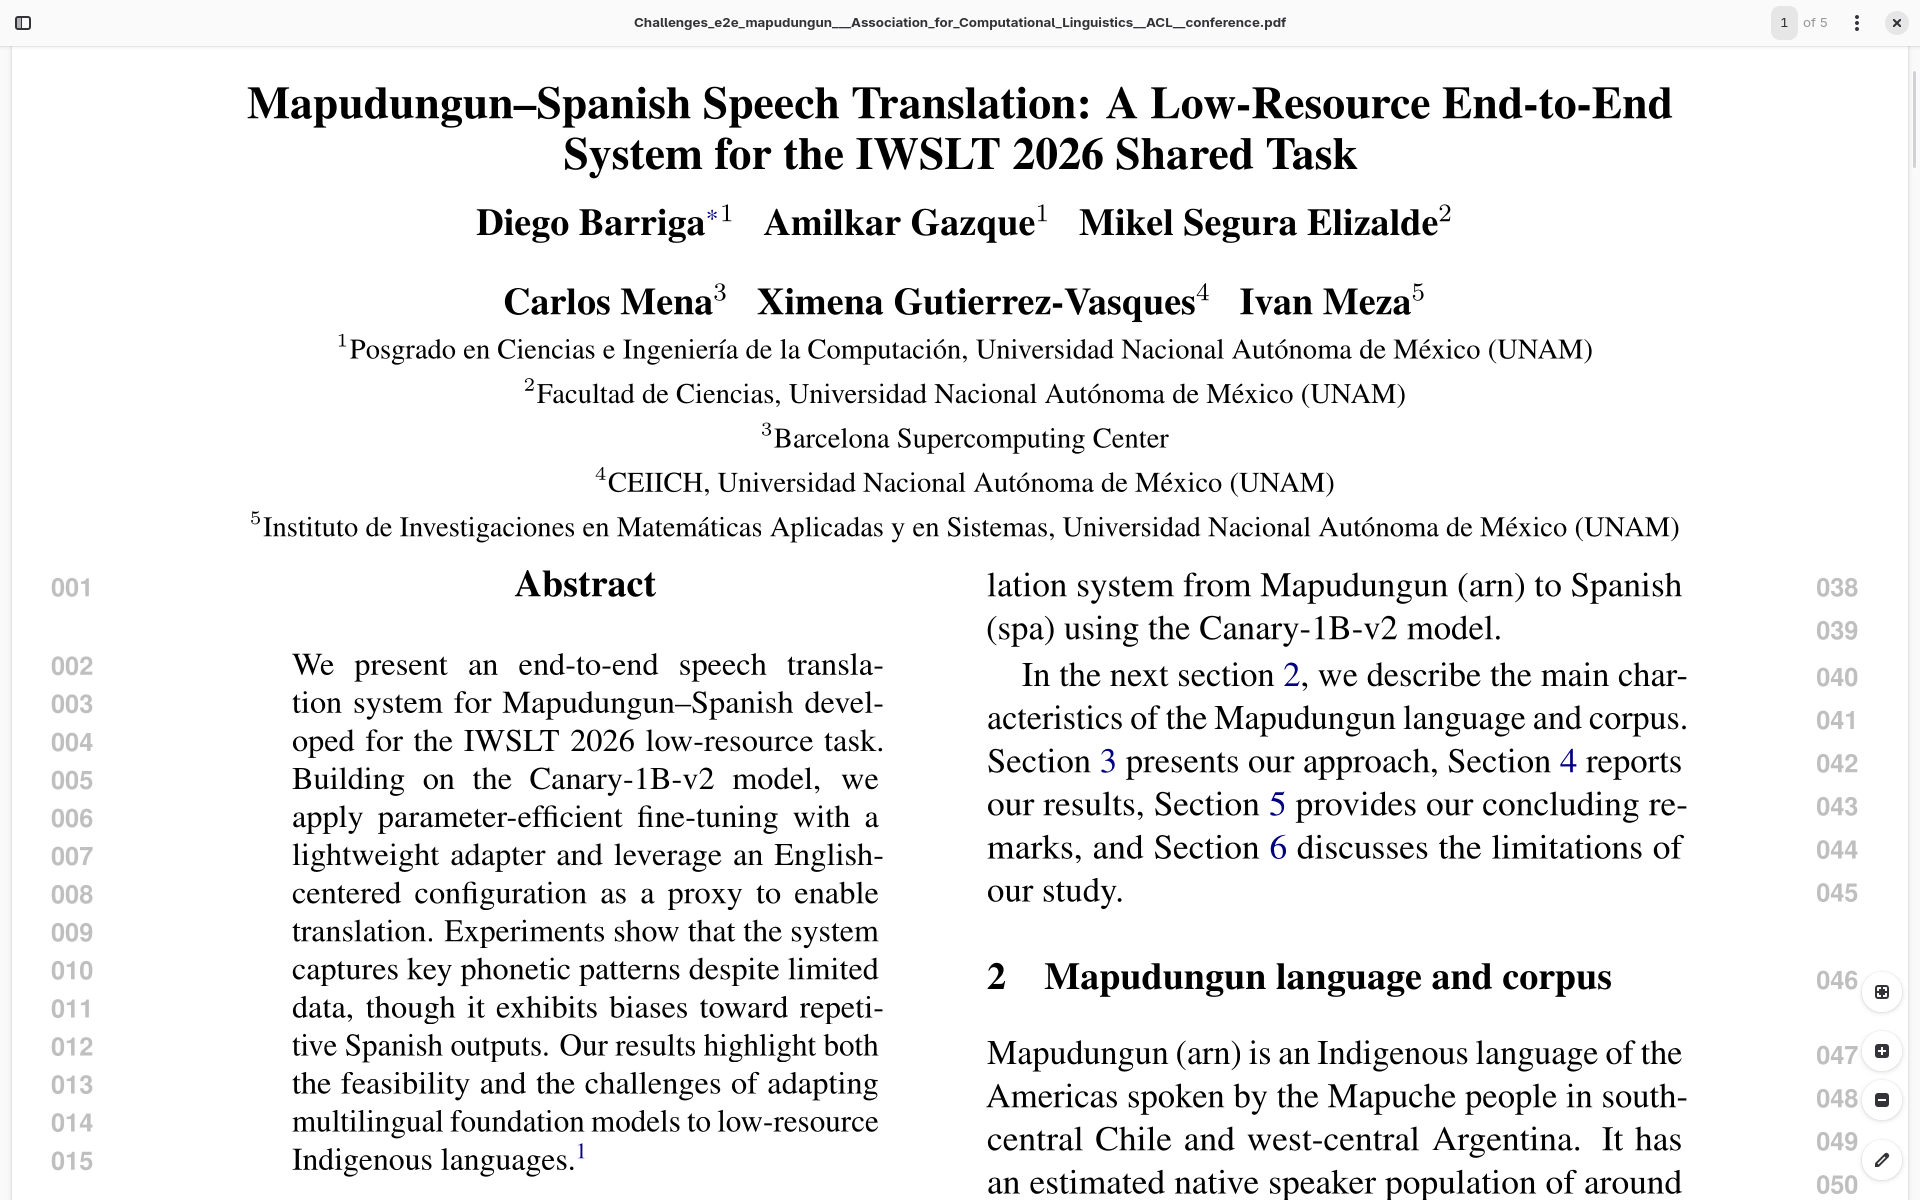
\includegraphics[width=\textwidth]{img/paper_cover.png}
        \caption{Portada del paper de la participación en IWSLT 2026.}
    \end{figure}
\end{frame}

\section{Conclusiones y trabajo futuro}

\begin{frame}{Conclusión}
    \begin{itemize}
        \item \textbf{Adaptación de Modelos:} Presentamos un enfoque para adaptar un modelo fundacional multilingüe y multitarea para la traducción de voz a texto de Mapudungun a Español.
        \item \textbf{Viabilidad Técnica:} A pesar de las limitaciones de recursos, la metodología logró capturar características fonéticas distintivas del Mapudungun, demostrando la eficacia del ajuste fino eficiente (\textit{PEFT}).
    \end{itemize}
\end{frame}

\begin{frame}{Trabajo futuro}

    \begin{itemize}
        \item Utilizar una lengua de bajos recursos mas cercana al Mapudungún como placeholder para el entrenamiento.
        \item Realizar experimentación adicional con diferentes estrategias de \textit{PEFT} y arquitecturas de modelos para mejorar el desempeño.
        \item Planeamos extender este marco de trabajo para desarrollar sistemas de traducción multilingües más amplios que incluyan otras lenguas originarias latinoamericanas, como el Quechua y el Náhuatl.
        \item El objetivo final es \alert{reducir la brecha tecnológica entre lenguas} de altos y bajos recursos, asegurando que estas voces estén representadas en las tecnologías de voz modernas.
    \end{itemize}
\end{frame}

\begin{frame}[allowframebreaks]{Referencias}
	\small
    \bibliographystyle{apalike}
    \bibliography{referencias}
\end{frame}

\begin{frame}
\centering
\Huge \textbf{¿Preguntas?}

\vspace{1cm}
\normalsize
\textbf{Contacto:} \\
Diego Barriga - \url{dbarriga@ciencias.unam.mx} \\
Edgar Gazque - \url{amilkar@ciencias.unam.mx}
\end{frame}
\end{document}
